% Template: Fabian Wenzelmann, 2016 - 2017

\documentclass[a4paper,
  twoside, % für Unterscheidung gerade / ungerade Seite
  headlines=2.1 % Anzahl der Zeilen im Kopf, wenn man mehr verwenden will erhöhen
  ]{scrartcl}
\AddToHook{cmd/section/before}{\clearpage}

\usepackage[
  margin=2cm,
  includefoot,
  footskip=35pt,
  includeheadfoot,
  headsep=0.5cm,
]{geometry}
\usepackage[utf8]{inputenc}
\usepackage{amsmath}
\usepackage{float}
\usepackage{amssymb}
\usepackage{amsthm}
\usepackage[automark,headsepline]{scrlayer-scrpage}
\usepackage{enumerate}
\usepackage[protrusion=true,expansion=true, kerning]{microtype} % Sieht damit einfach schöner aus
\usepackage{mathtools}

\raggedbottom
% nur für das Beispiel benötigt
\usepackage{lipsum}

\newcommand{\yourname}{Ioan Oleksii Kelier} % Weitere Autor*innen mittels \and Befehl einfügen
% \newcommand{\yourname}{Dein Name \\ \texttt{123456789} \and Anderer Name \\ \texttt{987654321}} % Hier ein Bsp mit Martikelnummern, auf jeden Fall \headingname anpassen (keine newlines)
\newcommand{\headingname}{Ioan Oleksii Kelier} % Namen wie sie im Kopf erscheinen, wenn zu lang z.B. nur Nachnamen verwenden
% Auch wenn man eine Trennung durch Kommata haben will hier die Namen erneut durch Kommata getrennt wiederholen
% \newcommand{\headingname}{Dein Name, Anderer Name} % Hier ein Beispiel für eine anders formatierte Liste
\newcommand{\lecture}{Algorithms notes}
\author{\yourname}
\title{\lecture}
\date{} % Wer ein Datum auf dem Dokument haben will hier eintragen, \today erstellt das heutige Datum

\pagestyle{scrheadings}
\setkomafont{pagehead}{\normalfont}
\lohead{\lecture\\\headingname}
\lehead{\lecture\\\headingname}

%------------------------------------------------------------------------------------------------------------------------------------------------
\begin{document}

\section*{General concepts}
Algorithm is considered to be correct if:

\begin{enumerate}
    \item Algorithm calculating the correct output for each input
    \item Algorithm is terminating
\end{enumerate}

\subsection*{Landau Symbols}

Some important notation:
\begin{enumerate}[(a)]
    \item $\mathbb{O}(n) := \{f(n) \;|\; \exists c, n_0 > 0 \; \forall n \geq n_0 \; : \; f(n) \leq c \cdot g(n)\}$
    \begin{itemize}
        \item \textbf{Means:} $f(n) \in \mathbb{O}(n)$ if there are constants $c$ and $n_0$ such that $f(n) \leq c \cdot g(n) \; \forall n \geq n_0$.
        \item \textbf{In simple terms:} $f(n) \leq g(n)$, asymptotically seen. $f(n)$ grows slower then $g(n)$.
    \end{itemize}

    \item $\Omega(n) := \{f(n) \; | \; \exists c, n_0 > 0 \; \forall n \geq n_0 \; : \; f(n) \geq c \cdot g(n)\}$ \\
     Means: Function $f(n) \in \Omega(n)$ if there exists constants $c$ and $n_0$ such that $f(n) \geq c \cdot g(n) \; \forall n \geq n_0$.
    


     
\end{enumerate}
%------------------------------------------------------------------------------------------------------------------------------------------------
\section*{Sorting algorithms}
    Some notation:
    \begin{itemize}
        \item Input array - $A$
    \end{itemize}
    \subsection*{Selection Sort}

    Key ideas of the algorithm: 
    \begin{itemize}
        \item Find the smallest element in array, switch it with the 1 element in array.
        \item Find the smallest element in array[2:n], switch it with the 2 element in array.
        \item \dots{}
    \end{itemize}
    Pseudo code:
    \begin{figure}[H]
        \centering
        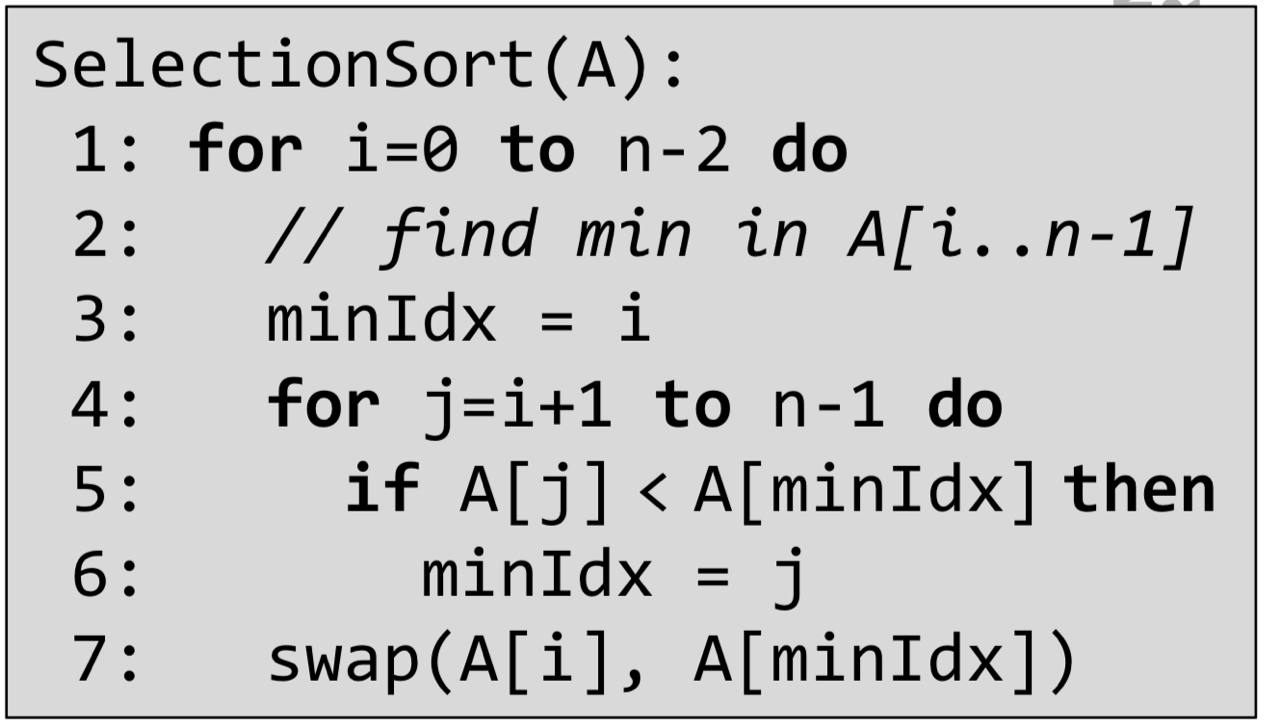
\includegraphics[width=0.3\linewidth]{image.png}
        \caption{Pseudo code for selection sort algorithm}
        \label{fig:enter-label}
    \end{figure}
    Key points from the lecture notes:
    \begin{itemize}
       \item  Main problem of the selection sort is that it becomes disproportionately slower with increasing size of the array.
       \item \textbf{Time complexity: $\mathbb{O}(n^{2})$.}
    \end{itemize}

    \clearpage
    \subsection*{Insertion sort}

    Key ideas of the algorithm:
    \begin{itemize}
        \item Gradually always add the next element to the already sorted part.
        
        \item We are swapping elements until either pos of current element is 0, which means that we reached start of our array, (for example part \textit{(d)} in Figure 2) or until we find element which is smaller then the current one (for example part \textit{(e)} in Figure 2).

        \item Efficiency depends on the following part: \textit{how nearly sorted the input array is}? It's important due to the fact that we may need to go all the way back to the last sorted element.

        \item \textbf{Time complexity: $\mathbb{O}(n^{2})$}
    \end{itemize}
    Pseudo code:
    \begin{figure}[H]
        \centering
        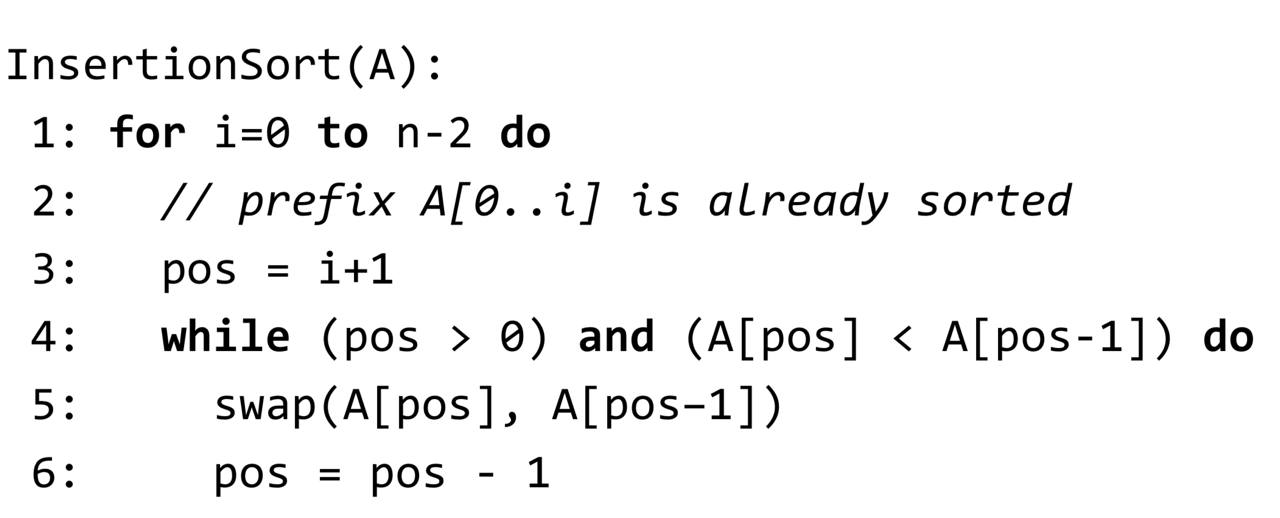
\includegraphics[width=0.5\linewidth]{insertion_sort_pseudocode.png}
        \caption{Insertion sort pseudo code}
        \label{fig:enter-label}
    \end{figure}
    Illustration of the algorithm:
    \begin{figure}[H]
        \centering
        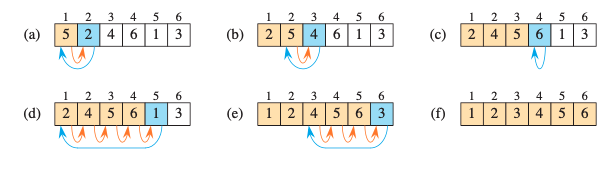
\includegraphics[width=0.7\linewidth]{insertion_sort_algo.png}
        \caption{Insertion sort algorithm}
        \label{fig:enter-label}
    \end{figure}

    \clearpage
    \subsection*{Quick Sort}

    Key idea:
    \begin{itemize}
        \item Divide array into two parts: \textbf{left} part with \textbf{smaller} elements, \textbf{right} part with bigger \textbf{elements}.
        \item Sort parts recursively
    \end{itemize}
    It's important to note, that it's unnecessary to create a new array for this, because it can be done in place with two variables (l and r):
    
    \begin{enumerate}
        \item Choose a pivot $x \in A$ and create two variables: $l = 0$ and $r = len(A) - 1$.
        \item Increment l until $A[l] > x$ (element should go to the right side)
        \item Decrement r until $A[l] <= x$ (element should go to the left side)
        \item Swap elements and do l += 1  and r -= 1 (move l to the left and r to the right)
        \item As soon as l == r stop
    \end{enumerate}
    Some information about the pivot element selection:
    \begin{enumerate}
        \item Size of both right and left sides depends on the pivot value.
        \item The smaller len(left) - left(right) the better the performance.
        \item Ideal (theor.) candidate for the pivot element is median (middle value in the sorted array), however it's not easy (read: time efficient?) to find it
        \item Some fixed element of the array is a bad choice, because it can lead to bad size of the parts
        \item Other possible candidates: median of three (or more) elements or random element in array \\
    \end{enumerate}

    One can see QuickSort as follows (Simplified):
    
    \begin{figure}[H]
        \centering
        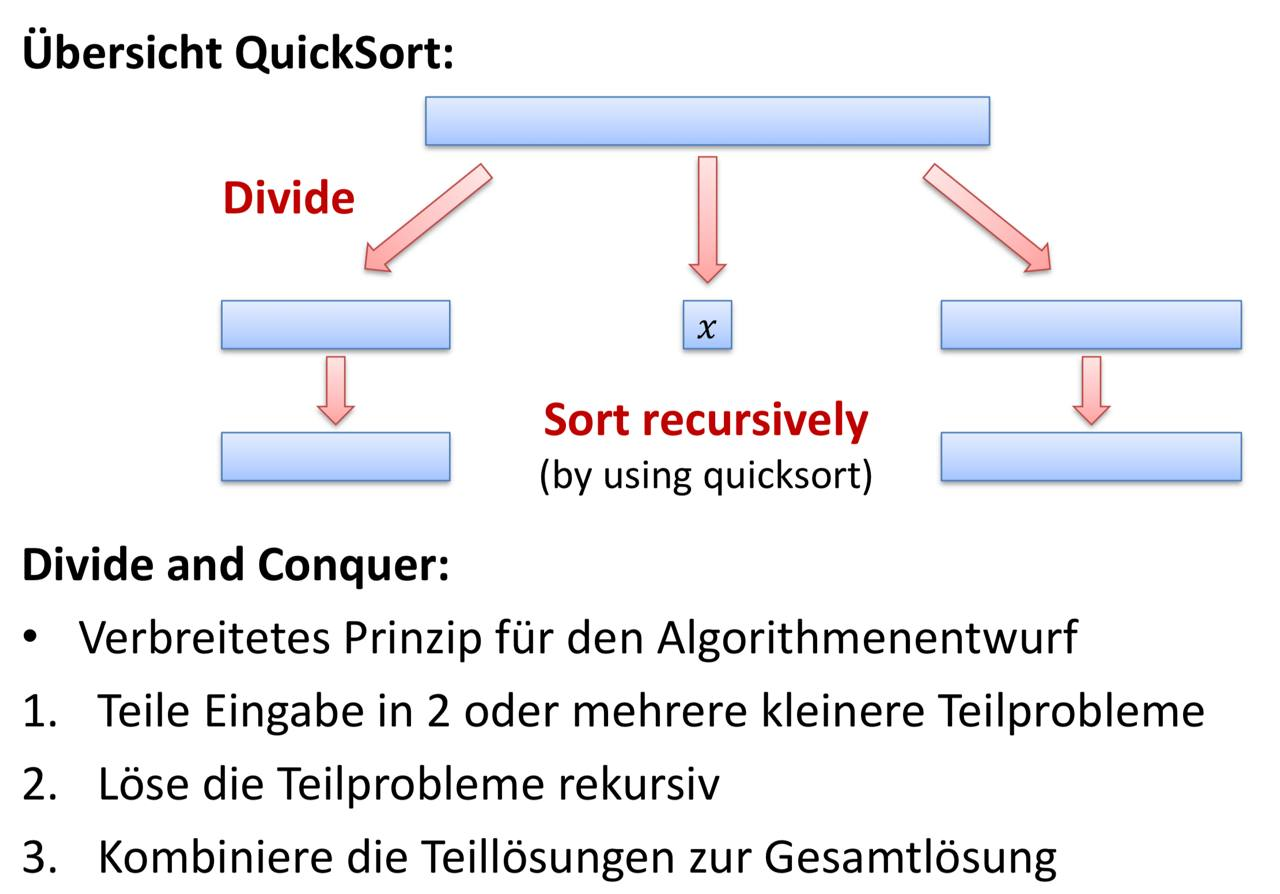
\includegraphics[width=0.5\linewidth]{quick_sort_simplyfied.png}
        \caption{Simplified representation of QS}
        \label{fig:enter-label}
    \end{figure}
    
    (I guees more info on QS later?)


    \clearpage
    \subsection*{Merge Sort}
    
    Key ideas:
    
    \begin{itemize}
        \item Based on Divide and Conquer principle.
        \item Consists of 3 main parts:
        \begin{itemize}
            \item \textbf{Divide}. Computes the middle of the subarray, which takes $\mathbb{O}(1)$.
            \item \textbf{Conquer}. Recursively solving 2 subproblems, each of size $\frac{n}{2}$, contributes $2T(\frac{n}{2})$ to the running time.
            \item \textbf{Combine}. Merge two subarrays. Takes $\mathbb{O}(1)$.
        \end{itemize}
        \item Recursive equation (proof in Cormen book pgs. 41 - 43):
        \begin{align*}
            T(n) = 2T\left(\frac{n}{2}\right) + \mathbb{O}(n)
        \end{align*}
        \item Resulting worst-case time complexity: $\mathbb{O}(nlg(n))$
    \end{itemize}
    
    One can think about Merge sort as follows:
    
    \begin{figure}[H]
        \centering
        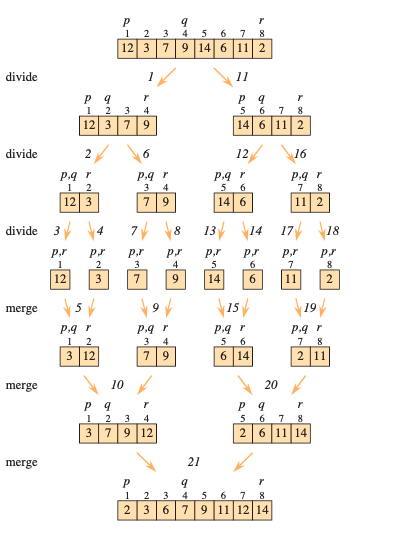
\includegraphics[width=0.5\linewidth]{merge_sort_example_cormen.png}
        \caption{MS example from Cormen book}
        \label{fig:enter-label}
    \end{figure}
    
    The heart of the algorithm is the \textit{merge} part. How does it work:
    
    \begin{itemize}
        \item We have two sorted arrays $A$ and $B$.
        \item Output - sorted array C with elements from A and B.
        \item Cost of one merge is $\mathbb{O}(n)$.
    \end{itemize}
    
    \begin{figure}[H]
            \centering
            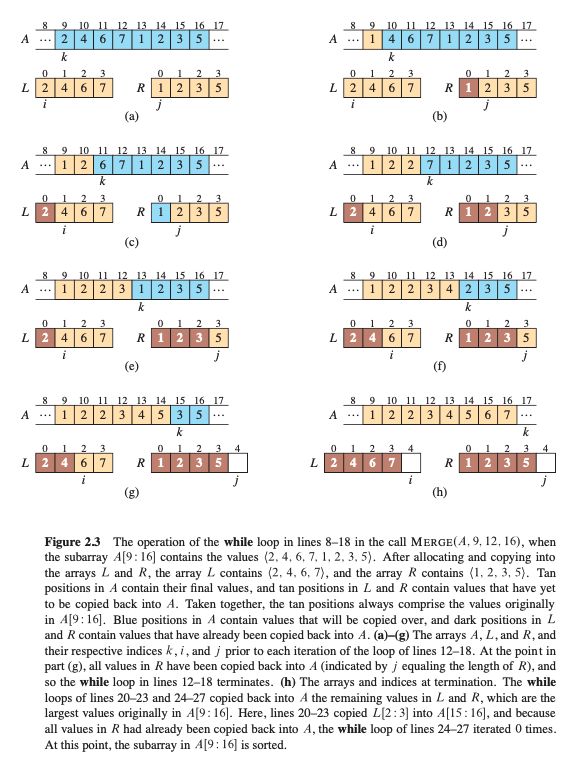
\includegraphics[width=0.7\linewidth]{merge_part_cormen.png}
            \caption{Merge part from Cormen book}
            \label{fig:enter-label}
    \end{figure}    
    
\end{document}